% id: 81-10
% book: 100발100중 3-2 기말 · 01 3-2 기말(원의 성질·통계·부록)
% section: 실전 문제 1회
% figure: crop:fig-81-10.png
% answer: ①
% answer_source: 답지(빠른정답)
% variant_level: 0 (원본 전사)
% 이 파일은 build.mjs 가 items.json 에서 만든다. 고칠 때는 items.json 을 고친다.
\smash{\raisebox{1.5mm}{\dmkichul{100발100중 3-2 기말 81쪽 10번 · 동영상}}}
\noindent\begin{minipage}[t]{0.58\linewidth}\vspace{0pt}\raggedright 그림은 어느 중학교 3학년 학생들의 중간고사와 기말고사의 국어 성적을 조사하여 나타낸 산점도이다. 이때 $\pt{A}$, $\pt{B}$, $\pt{C}$, $\pt{D}$, $\pt{E}$의 5명의 학생 중에서 두 성적의 차가 가장 큰 학생은?\end{minipage}\hfill\begin{minipage}[t]{0.4\linewidth}\vspace{0pt}\centering 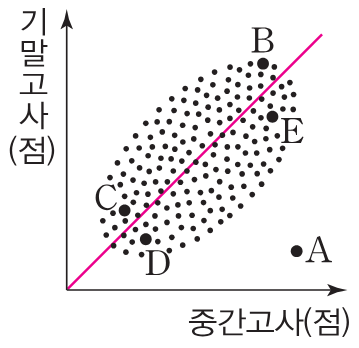
\includegraphics[width=86.0pt]{figures/fig-81-10.png}\end{minipage}\par
\begin{choices32}{$\pt{A}$}{$\pt{B}$}{$\pt{C}$}{$\pt{D}$}{$\pt{E}$}\end{choices32}
